\documentclass{article}
\usepackage{graphicx} % Required for inserting images
\usepackage{caption}
\usepackage{tabularx}
\usepackage{array}
\usepackage{booktabs}

\title{Relazione Linguistica Computazionale II - Tommaso Agostini}
\author{Tommaso Agostini}
\date{May 2026}

\renewcommand{\contentsname}{Indice}
\usepackage[a4paper, top=2.5cm, bottom=2.5cm, left=2.5cm, right=2.5cm]{geometry}

\begin{document}

\begin{titlepage}
    \centering
    \vspace*{\fill}

    {\Huge Linguistica Computazionale II\par}
    \vspace{1cm}

    {\LARGE Relazione di Progetto\par}
    \vspace{2cm}

    {\Large Tommaso Agostini - 692259\par}
    \vspace{0.5cm}

    {\large Anno Accademico 2025/2026\par}

    \vspace*{\fill}
\end{titlepage}

\tableofcontents
\newpage

\section{Introduzione}
Il presente report descrive il processo di sviluppo, addestramento e valutazione di modelli di classificazione per il task di \textit{machine-generated text detection}, formulato come un problema di classificazione binaria a livello di documento. L'obiettivo consiste nell'identificare l'origine di un testo, distinguendo tra contenuti scritti da autori umani (classe 0) e contenuti generati automaticamente da modelli linguistici (classe 1).

Per l'addestramento e la valutazione dei modelli è stato impiegato il dataset ufficiale del task \textit{Desegma-IT} (\textit{Detection and Segmentation of Machine Generated Text in Italian}), proposto nell'ambito della conferenza \textit{EVALITA 2026}.

\section{Costruzione dei dataset} Data la dimensione del corpus originale, è stato estratto un sottoinsieme dei dati per rendere gli esperimenti computazionalmente sostenibili. Il campionamento è stato effettuato in modo bilanciato, selezionando lo stesso numero di documenti per ciascuna classe. Il file di training è stato suddiviso in base all’etichetta di appartenenza. Successivamente, sono state estratte casualmente 1000 istanze per classe per la costruzione del training set. Gli indici dei documenti selezionati sono stati conservati per evitare sovrapposizioni con il validation set. Il validation set è stato ottenuto campionando ulteriori 500 documenti per classe tra le osservazioni rimanenti. Tutte le operazioni di campionamento sono state eseguite utilizzando il parametro \texttt{random\_state = 42}, al fine di garantire la riproducibilità degli esperimenti. Il test set è stato invece costruito a partire dal file \texttt{desegma-it.subTaskA.with\_labels.test}, contenente i documenti già corredati delle rispettive etichette. La composizione finale degli split è la seguente: training set (2000, 1000 per classe), validation set (1000, 500 per classe), test set (1000, 500 per classe).

\section{Preprocessing linguistico}
\label{sec:preprocessing}

Le annotazioni linguistiche sono state ottenute tramite Profiling-UD, eseguito su un archivio compresso contenente tutti i documenti del dataset.

Il tool ha prodotto due tipologie di output: (i) un insieme di file CoNLL-U, uno per documento, contenenti le annotazioni morfosintattiche secondo lo standard Universal Dependencies, e (ii) un file CSV contenente le feature di profiling linguistico a livello di documento.

I due output sono stati impiegati in modo distinto nei task successivi. I file CoNLL-U sono stati utilizzati nel Task 1 per la costruzione delle rappresentazioni basate su n-grammi di token, lemmi e POS tag, mentre il file CSV è stato utilizzato nel Task 2.

Per evitare disallineamenti tra gli split, training, validation e test set sono stati processati con un unico flusso. A tal fine, i documenti sono stati raccolti in una directory temporanea e rinominati mediante identificativi coerenti con lo split di appartenenza (ad esempio \texttt{train\_i.txt}, \texttt{val\_i.txt} e \texttt{test\_i.txt}), per poi essere compressi e forniti in input a Profiling-UD.

I file CoNLL-U sono stati successivamente processati tramite la funzione \texttt{estrai\_dati\_da\_conllu}. Da ciascun documento sono state estratte tre sequenze: token, lemmi e POS tag (UPOS).

Infine, gli split originali sono stati ricostruiti mediante gli identificativi dei file (\texttt{doc\_id}) mantenuti durante il preprocessing. Le sequenze ottenute (\texttt{tokens}, \texttt{lemmas} e \texttt{pos}) sono state convertite in stringhe compatibili con i vettorizzatori di scikit-learn e serializzate in formato Pickle per le successive fasi.

\section{Task 1: SVM lineari e n-grammi}

\subsection{Rappresentazione del testo e \textit{feature engineering}}

Il primo task ha previsto lo sviluppo di un classificatore basato su \texttt{LinearSVC}, utilizzando diverse rappresentazioni del testo a livello di n-grammi con l’obiettivo di modellare informazioni lessicali, morfologiche, sintattiche e sub-lessicali.

Sono state esplorate le seguenti configurazioni:
\begin{itemize}
    \item \textbf{Token:} unigrammi e bigrammi, per catturare il lessico esplicito del corpus.
    \item \textbf{Lemmi:} unigrammi e bigrammi, per ridurre la variabilità morfologica mantenendo l’informazione lessicale.
    \item \textbf{Part-of-Speech:} bigrammi e trigrammi, per modellare la struttura sintattica indipendentemente dal contenuto semantico.
    \item \textbf{Caratteri:} n-grammi di caratteri (3-5), per catturare pattern sub-lessicali, come prefissi, suffissi e regolarità ortografiche.
\end{itemize}

Per tutte le configurazioni è stata utilizzata la rappresentazione TF-IDF, al fine di ridurre l'influenza dei termini più frequenti e valorizzare quelli maggiormente discriminanti a livello di documento. Inoltre, è stato impostato il parametro $min\_df = 5$, che esclude dal vocabolario le feature presenti in meno di cinque documenti del training set. Questa scelta consente di ridurre il rumore e la dimensionalità dello spazio delle feature, eliminando pattern troppo rari e potenzialmente poco informativi e favorendo una migliore capacità di generalizzazione dei modelli.

\subsection{Selezione del modello tramite 5-fold cross-validation}

La selezione del modello è stata condotta sul training set mediante una \textit{5-fold cross-validation}, utilizzando il valore di Macro F1-score come riferimento.

\begin{table}[h]
\centering
\begin{tabular}{l l c}
\hline
\textbf{Configurazione} & \textbf{Livello Linguistico / Feature} & \textbf{Macro F1-score medio} \\
\hline
caratteri\_3\_5\_grammi & Caratteri & \textbf{0.9870} \\
token\_unigrammi\_bigrammi & Token & 0.9780 \\
lemmi\_bigrammi & Lemmi & 0.9735 \\
token\_unigrammi & Token & 0.9725 \\
lemmi\_unigrammi & Lemmi & 0.9710 \\
pos\_trigrammi & Part-of-Speech & 0.9605 \\
pos\_bigrammi & Part-of-Speech & 0.9430 \\
\hline
\end{tabular}
\caption{Risultati della 5-fold cross-validation ordinati per Macro F1-score medio decrescente.}
\label{tab:cv_results_svm}
\end{table}

I risultati medi ottenuti sono riportati in Tabella~\ref{tab:cv_results_svm}. Le prestazioni migliori si osservano per la rappresentazione basata su n-grammi di caratteri, che raggiunge una Macro-F1 score pari a 0.987. Tuttavia, anche le altre configurazioni ottengono risultati elevati, con valori superiori a 0.94, indicando che tutte le rappresentazioni considerate sono in grado di distinguere efficacemente tra testi umani e testi generati da modelli linguistici.

Considerate le elevate prestazioni ottenute, è stato effettuato un ulteriore tuning dell'iperparametro di regolarizzazione $C$ al fine di verificare la robustezza del modello e ridurre il rischio di overfitting. Valori più bassi di $C$ corrispondono a una regolarizzazione più forte, mentre valori più elevati consentono al modello di adattarsi maggiormente ai dati di training. Il valore $C = 0.1$ produce una Macro-F1 score pari a 0.977, mentre $C = 1.0$ raggiunge il valore massimo di 0.987 e viene pertanto selezionato come configurazione finale del modello.

Le rappresentazioni basate su token e lemmi ottengono prestazioni molto vicine a quelle della configurazione migliore, con Macro-F1 score rispettivamente pari a 0.9725 e 0.9710. Anche le rappresentazioni basate su POS mostrano risultati competitivi (0.9430--0.9605), sebbene leggermente inferiori. Nel complesso, le differenze osservate tra le diverse rappresentazioni risultano contenute, suggerendo che il compito di classificazione possa essere affrontato efficacemente mediante differenti livelli di rappresentazione linguistica.

\subsection{Valutazione finale su validation e test set}

Il modello più performante (n-grammi di caratteri) è stato poi valutato su validation e test set per verificarne la stabilità e la capacità di generalizzazione.

Sul validation set il modello ottiene prestazioni molto elevate, con Macro F1-score e accuracy prossimi a 0.99, indicando una forte coerenza tra le distribuzioni di training e validazione.

Sul test set si osserva invece una riduzione delle prestazioni, con Macro F1-score e accuracy pari a circa 0.85 (Tabella~\ref{tab:test_results}). L’analisi della matrice di confusione (Figura~\ref{fig:confusion_matrix_test}) evidenzia un’elevata precisione nella predizione della classe positiva (0.99), a fronte di una recall più bassa (0.71), dovuta a un numero significativo di falsi negativi. Questo comportamento suggerisce che il modello sia particolarmente conservativo nell’identificazione dei testi generati automaticamente, riuscendo a classificare correttamente solo una parte dei casi positivi.

La riduzione delle prestazioni sul test set può essere ricondotta a un possibile \textit{domain shift} tra validation e test set. Le feature basate su n-grammi di caratteri, pur efficaci nel dominio di addestramento, tendono a catturare pattern superficiali legati a stile, lessico e distribuzione del vocabolario, che risultano meno stabili in presenza di dati provenienti da una distribuzione differente.

\begin{figure}[h]
\centering

\begin{minipage}{0.48\textwidth}
\centering
\begin{tabular}{l c c c c}
\hline
\textbf{Classe} & \textbf{P} & \textbf{R} & \textbf{F1} & \textbf{Sup} \\
\hline
Umano (0) & 0.78 & 0.99 & 0.87 & 500 \\
LLM (1) & 0.99 & 0.71 & 0.83 & 500 \\
\hline
Accuracy & - & - & 0.85 & 1000 \\
Macro Avg & 0.88 & 0.85 & 0.85 & 1000 \\
Weighted Avg & 0.88 & 0.85 & 0.85 & 1000 \\
\hline
\end{tabular}
\captionof{table}{Prestazioni sul test set (n-grammi di caratteri)}
\label{tab:test_results}
\end{minipage}
\hfill
\begin{minipage}{0.48\textwidth}
\centering
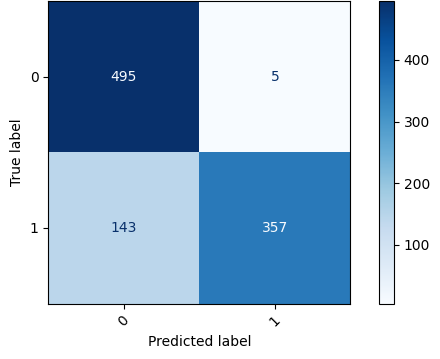
\includegraphics[width=0.8\textwidth]{figures/task1_matrix_test.png}
\captionof{figure}{Matrice di confusione sul test set (n-grammi di caratteri)}
\label{fig:confusion_matrix_test}
\end{minipage}
\end{figure}

\section{Task 2: SVM lineari e informazioni linguistiche non lessicali}

\subsection{Descrizione del task e delle feature utilizzate}

Il secondo task utilizza un classificatore LinearSVC basato su feature linguistiche non lessicali, con l’obiettivo di modellare lo stile e la struttura dei testi indipendentemente dal contenuto semantico. Le feature, derivate dal processo di \textit{linguistic profiling} (Sezione~\ref{sec:preprocessing}) e già allineate agli split del dataset, sono 142 per documento e coprono tre principali livelli di analisi linguistica:

\begin{itemize}
    \item \textbf{Stilometria e complessità}: misure come lunghezza media dei token e ricchezza lessicale;
    \item \textbf{Morfosintassi}: distribuzione delle categorie grammaticali (UPOS);
    \item \textbf{Struttura sintattica}: informazioni sulle relazioni di dipendenza e sulla complessità delle costruzioni sintattiche.
\end{itemize}

Le feature sono state normalizzate mediante \texttt{StandardScaler}, per renderle confrontabili e ridurre l’influenza di variabili con range numerico più ampio sulla costruzione del margine decisionale della SVM.
La configurazione iniziale utilizza $C=1.0$, confrontata con una variante più regolarizzata ($C=0.1$) per verificarne la robustezza. La modifica non comporta variazioni significative nelle prestazioni su training, validation e test set (la Macro-F1 sul training set passa da 0.98 a 0.97); pertanto, è stato mantenuto $C=1.0$.

\begin{figure}[h]
\centering
\begin{minipage}[b]{0.32\textwidth}
\centering
\textbf{Training}\\[2mm]
\begin{tabular}{l c c c}
\hline
 & \textbf{P} & \textbf{R} & \textbf{F1} \\
\hline
0 & 0.98 & 0.98 & 0.98 \\
1 & 0.98 & 0.98 & 0.98 \\
\hline
Accuracy & & & 0.98 \\
Macro & & & 0.98 \\
Weighted & & & 0.98 \\
\hline
\end{tabular}
\end{minipage}
\hfill
\begin{minipage}[b]{0.32\textwidth}
\centering
\textbf{Validation}\\[2mm]
\begin{tabular}{l c c c}
\hline
 & \textbf{P} & \textbf{R} & \textbf{F1} \\
\hline
0 & 0.94 & 0.94 & 0.94 \\
1 & 0.94 & 0.94 & 0.94 \\
\hline
Accuracy & & & 0.94 \\
Macro & & & 0.94 \\
Weighted & & & 0.94 \\
\hline
\end{tabular}
\end{minipage}
\hfill
\begin{minipage}[b]{0.32\textwidth}
\centering
\textbf{Test}\\[2mm]
\begin{tabular}{l c c c}
\hline
 & \textbf{P} & \textbf{R} & \textbf{F1} \\
\hline
0 & 0.84 & 0.93 & 0.88 \\
1 & 0.92 & 0.82 & 0.87 \\
\hline
Accuracy & & & 0.88 \\
Macro & & & 0.88 \\
Weighted & & & 0.88 \\
\hline
\end{tabular}
\end{minipage}
\caption{Prestazioni del modello LinearSVC ($C=1.0$) sui set di training, validation e test. La tabella riporta precision, recall e F1-score per classe, oltre ad accuracy e alle medie macro e pesata dell'F1-score.}
\label{tab:svc_reports}
\end{figure}



I risultati nella Tabella~\ref{tab:svc_reports} evidenziano una buona capacità del modello di generalizzare rappresentazioni basate su tratti sintattici e stilistici astratti. Le prestazioni risultano elevate sul validation set (Macro F1 = 0.94), mentre sul test set si osserva una riduzione contenuta (Macro F1 = 0.88), inferiore rispetto ai modelli basati su feature lessicali. Sul test set, il modello mostra un comportamento complessivamente bilanciato, con precisione pari a 0.92 per la classe positiva e recall pari a 0.82, indicando una lieve tendenza conservativa nella classificazione dei testi generati automaticamente.

\subsection{Analisi dei documenti di difficile classificazione}

Per analizzare i limiti del modello e le aree di ambiguità tra le classi, è stata considerata la distanza dei documenti del test set dall’iperpiano decisionale della SVM. Attraverso la funzione \texttt{decision\_function()}, ogni istanza è associata a un punteggio continuo: il segno del valore indica la classe predetta (negativo per la classe 0 e positivo per la classe 1), mentre il valore assoluto ne rappresenta la confidenza. Valori prossimi allo zero corrispondono a esempi per i quali il classificatore mostra maggiore incertezza decisionale.
La Tabella~\ref{tab:doc_incerti} riporta le cinque istanze del test set con distanza minima dall’iperpiano decisionale.

\begin{table}[htbp]
\centering
\begin{tabularx}{\textwidth}{c c c c X}
\hline
\textbf{ID} & \textbf{Score} & \textbf{True} & \textbf{Pred} & \textbf{Estratto} \\
\hline

411 & -0.0061 & 1 & 0 & Una qualificazione che, francamente, lascia un po’ di amaro in bocca. Non per la prestazione del Feyenoord, squadra solida e mai doma, ma per quella dei giallorossi. [...] \\

539 & -0.0071 & 0 & 0 & Culle di pelliccia, quindi, amiche del respiro dei bebè. Perché il rischio di avere l'asma a 6 anni crolla di quasi l'80\% e del 40\% la probabilità di soffrirne a 10. [...] \\

620 & 0.0138 & 1 & 1 & Una cifra considerevole, che si somma a quelle registrate negli anni precedenti, che dimostrano la grande passione civica che anima i donatori, gruppi e singoli [...] \\

666 & -0.0335 & 1 & 0 & According to Amnesty, sino al 2023 sarebbero state pi\`u di 20mila le persone respinte [...] in\textbf{[caratteri bengalesi]} e violente [...] senza\textbf{[caratteri arabi]} chance di Understanding [...] \\

60 & 0.0341 & 0 & 1 & Ma il trauma rimane. A prendere di mira la turista 12enne è stato un ecuadoriano di cinquantadue anni, già noto alle forze dell'ordine per altri reati [...] \\

\hline
\end{tabularx}
\caption{Esempi di documenti del test set con minima distanza dall’iperpiano decisionale (modello SVM con feature non lessicali)}
\label{tab:doc_incerti}
\end{table}

L’analisi qualitativa di questi casi evidenzia come l’incertezza del modello sia spesso riconducibile a un disallineamento tra la classe reale del documento e le sue caratteristiche stilistiche e sintattiche, che influenzano le feature estratte.

Il falso negativo relativo all’istanza 411 (testo generato classificato come umano) mostra come il modello di linguaggio sia in grado di replicare efficacemente lo stile del giornalismo sportivo, attraverso l’uso di espressioni idiomatiche e variazioni sintattiche che contribuiscono a una forte somiglianza con la scrittura naturale.

Al contrario, il falso positivo identificato nell’istanza 60 (testo umano classificato come generato) è caratterizzato da uno stile giornalistico altamente regolare e fattuale. Tale struttura, tipica di testi informativi, può essere erroneamente interpretata dal modello come segnale di generazione automatica.

Nel caso dell’istanza 666 (falso negativo), che presenta artefatti testuali e contaminazioni di caratteri appartenenti ad alfabeti differenti, è plausibile che tali anomalie abbiano compromesso l’estrazione delle feature sintattiche basate sul parsing (ad esempio dipendenze e tag POS), introducendo pattern irregolari assimilabili alla variabilità tipica di testi umani.

Nel complesso, questi risultati indicano che le feature linguistiche non lessicali costituiscono indicatori robusti a livello globale, ma possono risultare sensibili a stili di scrittura estremamente controllati o, al contrario, a generazioni che inducono forte rumore superficiale nel testo.

\subsection{Analisi delle feature più rilevanti}

\begin{table}[h]
\centering

\begin{minipage}{0.48\textwidth}
\centering
\begin{tabular}{lr}
\toprule
\textbf{Feature} & \textbf{Peso} \\
\midrule
n\_tokens & -2.4195 \\
dep\_dist\_advmod & 1.8747 \\
upos\_dist\_ADV & -1.5253 \\
lexical\_density & -1.4572 \\
n\_prepositional\_chains & 1.3093 \\
ttr\_form\_chunks\_200 & -1.2971 \\
dep\_dist\_det & -1.2332 \\
upos\_dist\_NUM & -1.1211 \\
upos\_dist\_PUNCT & 1.0166 \\
upos\_dist\_PRON & -0.9998 \\
\bottomrule
\end{tabular}
\end{minipage}
\hfill
\begin{minipage}{0.48\textwidth}
\centering
\begin{tabular}{lr}
\toprule
\textbf{Feature} & \textbf{Peso} \\
\midrule
upos\_dist\_DET & 0.9307 \\
dep\_dist\_flat:foreign & -0.8940 \\
dep\_dist\_case & -0.7998 \\
upos\_dist\_VERB & -0.7752 \\
avg\_prepositional\_chain\_len & -0.7629 \\
avg\_subordinate\_chain\_len & -0.7153 \\
upos\_dist\_ADP & 0.6061 \\
upos\_dist\_PROPN & -0.5876 \\
dep\_dist\_acl:relcl & 0.5424 \\
dep\_dist\_nsubj & 0.5011 \\
\bottomrule
\end{tabular}
\end{minipage}

\caption{Top 20 feature per peso assoluto nella SVM lineare (ordinate per valore assoluto decrescente). Un peso negativo favorisce la classificazione nella classe umana, mentre un peso positivo favorisce la classificazione nella classe artificiale.}
\label{tab:top_features}
\end{table}

L'analisi dei pesi evidenzia pattern linguistici coerenti tra le due classi.

Per la classe umana (pesi negativi), le feature più rilevanti includono indicatori di lunghezza e ricchezza testuale come il numero di token (\texttt{n\_tokens}), la densità lessicale (\texttt{lexical\_density}) e la variabilità del vocabolario (\texttt{ttr\_form\_chunks\_200}). A livello morfosintattico emergono una maggiore presenza di avverbi, pronomi e nomi propri, oltre a catene subordinate e preposizionali mediamente più lunghe e a una maggiore incidenza della relazione di dipendenza dei determinanti (\texttt{dep\_dist\_det}).

Per la classe artificiale (pesi positivi), risultano invece più influenti caratteristiche riconducibili a una maggiore strutturazione sintattica del testo: una maggiore incidenza di modificatori avverbiali (\texttt{dep\_dist\_advmod}), determinanti (\texttt{upos\_dist\_DET}) e punteggiatura, insieme a una frequenza più elevata di catene preposizionali (\texttt{n\_prepositional\_chains}), costruzioni relative (\texttt{dep\_dist\_acl:relcl}) e soggetti espliciti (\texttt{dep\_dist\_nsubj}).

Nel complesso, queste evidenze suggeriscono che la separazione tra le due classi 
sia guidata da differenze stilistiche e strutturali piuttosto che da singoli 
segnali lessicali isolati.


\section{Task 3: SVM lineari e word embeddings}

Questa sezione esplora l’utilizzo di rappresentazioni vettoriali dense basate su \textit{word embeddings} statici pre-addestrati sul corpus itWaC (dimensione 128). Poiché tali embedding sono definiti a livello di parola, è necessario applicare strategie di aggregazione per ottenere rappresentazioni a livello di documento di dimensione fissa, compatibili con LinearSVC.

Gli embedding sono stati convertiti nel formato \texttt{float32} e organizzati in una struttura a dizionario. I token vengono normalizzati mediante l’uso di espressioni regolari: gli URL vengono sostituiti con la stringa \texttt{\_\_\_URL\_\_\_}, i numeri vengono mappati su un token dedicato \texttt{@Dg}, le parole eccessivamente lunghe vengono limitate e la capitalizzazione viene gestita in modo standardizzato. Nel caso in cui il token normalizzato non sia ancora presente nel vocabolario, viene convertito in minuscolo.

\subsection{Strategie di aggregazione e risultati sul validation set}

Per individuare la rappresentazione vettoriale più efficace per ciascun documento, sono stati confrontati tre diversi metodi di aggregazione applicati a due configurazioni di token filtrati in base al POS-tag. La prima configurazione (A) include i token appartenenti alle categorie NOUN, ADJ e VERB, mentre la seconda configurazione (B) considera VERB, NOUN, INTJ e DET.

Ogni configurazione è stata valutata all’interno di una pipeline composta da \texttt{StandardScaler} e \texttt{LinearSVC}, utilizzando \texttt{random\_state=42} e \texttt{max\_iter=10000} per garantire la riproducibilità dei risultati.

\begin{table}[h]
\centering
\begin{tabular}{llc}
\toprule
\textbf{Pooling} & \textbf{POS} & \textbf{Macro-F1} \\
\midrule
Sum & B (VERB, NOUN, INTJ, DET) & \textbf{0.947} \\
Sum & A (NOUN, ADJ, VERB) & 0.944 \\
Mean & A (NOUN, ADJ, VERB) & 0.931 \\
Mean & B (VERB, NOUN, INTJ, DET) & 0.930 \\
Max & B (VERB, NOUN, INTJ, DET) & 0.892 \\
Max & A (NOUN, ADJ, VERB) & 0.890 \\
\bottomrule
\end{tabular}
\caption{Confronto delle prestazioni per le diverse strategie di aggregazione (pooling) applicate ai word embedding sul validation set}
\label{tab:pooling_results}
\end{table}

I risultati riportati nella Tabella~\ref{tab:pooling_results} evidenziano che la strategia basata su \textit{Sum Pooling} ottiene in generale le prestazioni più elevate rispetto alle altre configurazioni, con risultati consistenti su entrambe le varianti di filtraggio morfosintattico. Questo comportamento suggerisce che le informazioni legate alla norma dei vettori e alla lunghezza del documento possano contribuire in modo rilevante alla separazione nello spazio delle rappresentazioni, rispetto alle formulazioni basate su \textit{Mean Pooling} e \textit{Max Pooling}, che mostrano prestazioni inferiori.

Tra le configurazioni considerate, la Configurazione B risulta la più efficace, raggiungendo il valore massimo di Macro-F1 pari a 0.947. L’inclusione di categorie di POS più eterogenee, comprendenti anche elementi funzionali ed espressivi, sembra fornire segnali aggiuntivi utili alla classificazione, rispetto a un insieme limitato al solo lessico di contenuto.

La configurazione basata su \textit{Sum Pooling} con filtro POS B è stata quindi selezionata per la valutazione finale sul test set, in quanto associata alle migliori prestazioni sul validation set (Macro-F1 = 0.947) e a una buona capacità di generalizzazione (Macro-F1 = 0.88 sul test set).

\subsection{Valutazione finale sul test set}

Il modello selezionato è stato valutato sul test set e ha ottenuto una Macro-F1 pari a 0.88 e un’accuracy complessiva pari a 0.88. I risultati dettagliati sono riportati in Tabella~\ref{tab:embeddings_test_report}, mentre la matrice di confusione è mostrata in Figura~\ref{fig:embeddings_confusion}.

L’analisi delle prestazioni evidenzia un bilanciamento relativamente equilibrato tra le due classi. In particolare, la classe umana (0) presenta una recall pari a 0.92 e una precisione di 0.85, mentre la classe artificiale (1) raggiunge una precisione di 0.91 e una recall di 0.84.

Nel complesso, il modello mostra una buona capacità di generalizzazione, con una riduzione attesa delle prestazioni rispetto al valore ottimale osservato su validation set. Questo comportamento può essere ricondotto al fatto che gli embedding statici tendono a catturare principalmente relazioni semantiche globali basate su co-occorrenze lessicali, risultando più sensibili a variazioni distribuzionali tra training e test set.

In questo contesto, la combinazione selezionata si conferma una scelta robusta. Il \textit{Sum Pooling} consente di preservare implicitamente informazioni legate alla rappresentazione vettoriale e alla lunghezza del documento, mentre l'insieme di POS della Configurazione B introduce segnali sintattici e stilistici aggiuntivi, contribuendo a mitigare parzialmente i limiti degli embedding statici in scenari di dominio non perfettamente allineato.

\begin{figure}[h]
\centering

\begin{minipage}{0.48\textwidth}
\centering
\begin{tabular}{l c c c c}
\hline
\textbf{Classe} & \textbf{P} & \textbf{R} & \textbf{F1} & \textbf{Sup} \\
\hline
Umano (0) & 0.85 & 0.92 & 0.88 & 500 \\
LLM (1) & 0.91 & 0.84 & 0.87 & 500 \\
\hline
Accuracy & - & - & 0.88 & 1000 \\
Macro Avg & 0.88 & 0.88 & 0.88 & 1000 \\
Weighted Avg & 0.88 & 0.88 & 0.88 & 1000 \\
\hline
\end{tabular}
\captionof{table}{Prestazioni del modello LinearSVC sul test set (configurazione: vector\_sum\_B)}
\label{tab:embeddings_test_report}
\end{minipage}
\hfill
\begin{minipage}{0.48\textwidth}
\centering
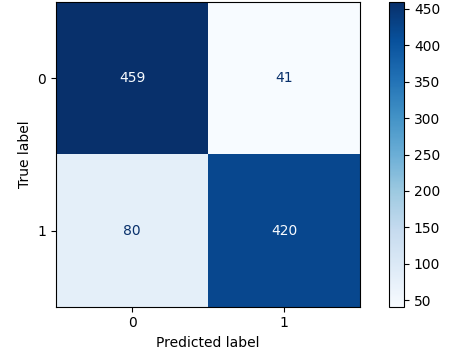
\includegraphics[width=0.8\textwidth]{figures/task3_matrix_test.png}
\captionof{figure}{Matrice di confusione sul test set (vector\_sum\_B)}
\label{fig:embeddings_confusion}
\end{minipage}
\end{figure}

\section{Task 4: Fine-tuning di un modello linguistico neurale}

Il quarto task affronta il problema della \textit{machine-generated text detection} mediante un modello neurale basato su architettura Transformer. A differenza degli approcci precedenti, fondati su rappresentazioni sparse, feature sintattiche esplicite ed embedding statici, questo esperimento si basa sul fine-tuning di un modello linguistico pre-addestrato.

Il modello selezionato è \texttt{dbmdz/bert-base-italian-cased}, una variante di BERT composta da 12 layer e pre-addestrata su un ampio corpus in lingua italiana. Grazie al meccanismo di self-attention bidirezionale, il modello è in grado di costruire rappresentazioni contestuali dei token, permettendo di catturare dipendenze sintattiche e regolarità distribuzionali.

\subsection{Configurazione e pre-elaborazione}

I dataset utilizzati coincidono con quelli degli esperimenti precedenti. Per garantire la riproducibilità degli esperimenti sono stati fissati i \textit{seed} di Python, NumPy e PyTorch, mentre l’addestramento è stato eseguito in ambiente GPU CUDA.

Il testo grezzo è stato fornito direttamente al tokenizer del modello, senza ulteriori fasi di normalizzazione manuale. La tokenizzazione è avvenuta tramite WordPiece, producendo le rappresentazioni \texttt{input\_ids} e \texttt{attention\_mask}. La sequenza è stata quindi adattata mediante operazioni di padding e truncation fino a una lunghezza massima di 512 token.

Il fine-tuning è stato eseguito per 3 epoche utilizzando un \textit{learning rate} pari a $5 \times 10^{-6}$, un \textit{batch size} di 8 e un \textit{weight decay} di 0.01. La selezione del modello finale è stata effettuata sulla base delle prestazioni in termini di F1-score sul validation set, salvando il checkpoint con le performance migliori.

\subsection{Addestramento}

Durante il fine-tuning, le metriche sono state monitorate tramite il \texttt{Trainer} di Hugging Face. La Tabella~\ref{tab:bert_training} riporta le prestazioni sul validation set al termine di ciascuna epoca.

\begin{table}[htbp]
\centering
\footnotesize % Rimpicciolisce leggermente il font per far stare tutto comodamente
\setlength{\tabcolsep}{4pt} % Riduce lo spazio orizzontale tra le colonne

\begin{minipage}[t]{0.48\textwidth}
\centering
\caption{Metriche di addestramento e validazione per epoca durante il fine-tuning di BERT.}
\label{tab:bert_training}
\begin{tabular}{l c c c c}
\hline
\textbf{Epoca} & \textbf{Train Loss} & \textbf{Val Loss} & \textbf{F1} & \textbf{Acc} \\
\hline
1 & 0.3748 & 0.2075 & 0.9419 & 0.9420 \\
2 & 0.1068 & 0.1118 & 0.9730 & 0.9730 \\
3 & 0.0755 & 0.1032 & 0.9770 & 0.9770 \\
\hline
\end{tabular}
\end{minipage}
\hfill
\begin{minipage}[t]{0.48\textwidth}
\centering
\caption{Risultati (BERT fine-tuned) sul test set.}
\label{tab:bert_test}
\begin{tabular}{l c c c c}
\hline
\textbf{Classe} & \textbf{P} & \textbf{R} & \textbf{F1} & \textbf{Sup} \\
\hline
Umano (0) & 0.96 & 0.87 & 0.91 & 500 \\
LLM (1) & 0.88 & 0.97 & 0.92 & 500 \\
\hline
Accuracy & - & - & 0.92 & 1000 \\
Macro Avg & 0.92 & 0.92 & 0.92 & 1000 \\
Weighted Avg & 0.92 & 0.92 & 0.92 & 1000 \\
\hline
\end{tabular}
\end{minipage}
\end{table}

\vspace{1em}
\noindent
\begin{minipage}[c]{0.55\textwidth}
L'andamento delle loss function, visualizzato in Figura~\ref{fig:loss_curve_bert}, mostra una convergenza regolare e stabile. La training loss diminuisce progressivamente in modo marcato, assestandosi a circa 0.077 al termine del processo, mentre la validation loss decresce parallelamente fino a raggiungere il suo minimo globale alla terza epoca (0.1067). La forte vicinanza tra le due curve nelle fasi finali e l'assenza di un'inversione di tendenza della validation loss suggerisce l'assenza di segnali di overfitting, indicando che il modello ha appreso in modo stabile le regolarità discriminative tra testi umani e testi generati da modelli linguistici.

Le prestazioni raggiungono il valore massimo alla terza epoca (Macro F1 = 0.977), che viene pertanto selezionata come configurazione finale del modello.
\end{minipage}
\hfill
\begin{minipage}[c]{0.40\textwidth}
\centering
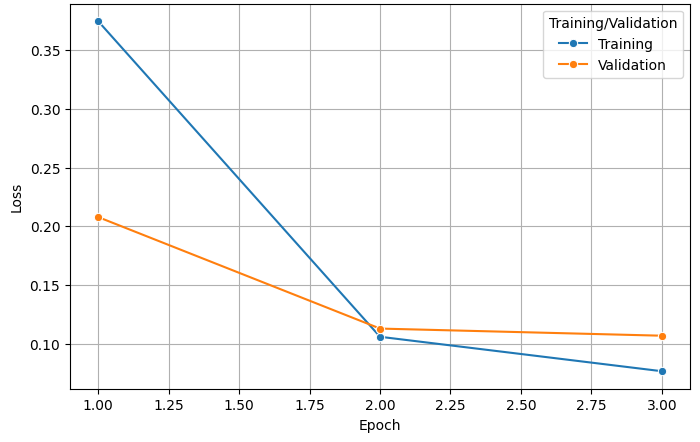
\includegraphics[width=\textwidth]{figures/curve_loss.png}
\captionof{figure}{Andamento della Training Loss e della Validation Loss durante le epoche di fine-tuning.}
\label{fig:loss_curve_bert}
\end{minipage}
\vspace{1em}

\subsection{Valutazione sul test set}
Il modello selezionato è stato valutato sul test set tramite \texttt{trainer.predict()}. I risultati metrici complessivi sono riportati in Tabella~\ref{tab:bert_test}, mentre la distribuzione esatta delle predizioni è analizzabile attraverso la matrice di confusione illustrata in Figura~\ref{fig:conf_matrix_test}.
Il modello ottiene prestazioni complessivamente elevate, con Macro F1 e accuracy pari a 0.92. Osservando i valori assoluti della matrice di confusione, emerge un comportamento asimmetrico nelle predizioni: su 500 testi generati da LLM, ben 483 vengono classificati correttamente, registrando appena 17 falsi negativi per la classe artificiale. Al contrario, la classe umana risulta maggiormente soggetta a confusione, con 435 testi riconosciuti correttamente e 65 testi umani erroneamente etichettati come generati da macchina (falsi positivi).

\vspace{1em} % Aggiunge un po' di spazio prima del blocco
\noindent
\begin{minipage}[c]{0.55\textwidth}
Questo squilibrio è coerente con le metriche riportate nella Tabella~\ref{tab:bert_test}: la classe artificiale presenta una recall elevata (0.97) ma una precision più contenuta (0.88), mentre la classe umana mostra il comportamento opposto, con una precision più alta (0.96) e una recall inferiore (0.87).

Nel complesso, il modello risulta più efficace nell’identificare i testi generati da LLM rispetto ai testi umani, che tendono a essere occasionalmente classificati con 1 quando caratterizzati da strutture sintattiche particolarmente regolari o poco variabili.
\end{minipage}
\hfill
\begin{minipage}[c]{0.35\textwidth}
\centering
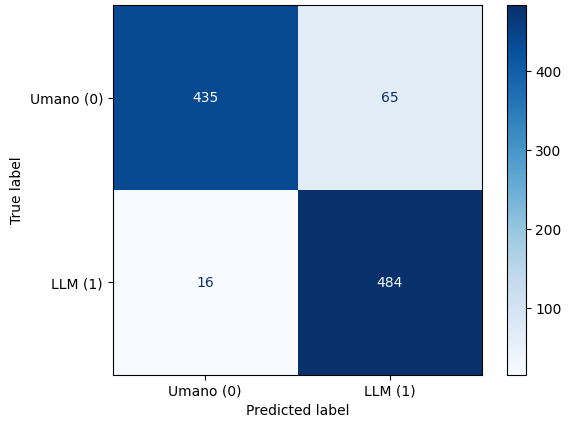
\includegraphics[width=\textwidth]{figures/task4_matrix_test.png}
\captionof{figure}{Matrice di confusione sul test set (BERT)}
\label{fig:conf_matrix_test}
\end{minipage}
\vspace{1em} % Aggiunge un po' di spazio dopo il blocco




\section{Conclusioni}

In questo lavoro sono stati sviluppati e confrontati quattro approcci per il task di \textit{machine-generated text detection} in lingua italiana, utilizzando il dataset ufficiale Desegma-IT di EVALITA 2026. Gli esperimenti hanno permesso di valutare l'efficacia di diverse tipologie di rappresentazione testuale, dalle feature sparse basate su n-grammi fino a modelli neurali contestuali basati su Transformer.

Tutti gli approcci considerati hanno ottenuto prestazioni significativamente superiori alla baseline casuale, confermando la presenza di segnali linguistici utili alla discriminazione tra testi scritti da autori umani e testi generati automaticamente. La Tabella~\ref{tab:final_results} riassume le prestazioni delle migliori configurazioni per ciascun task, confrontando i risultati sul validation set e sul test set.

\begin{table}[h]
\centering
\begin{tabular}{lcc}
\hline
\textbf{Configurazione} & \textbf{Validation F1} & \textbf{Test F1} \\
\hline
Task 1 - SVM + n-grammi di caratteri (3-5) & 0.987 & 0.850 \\
Task 2 - SVM + feature linguistiche Profiling-UD & 0.940 & 0.880 \\
Task 3 - SVM + embedding statici (Sum Pooling B) & 0.947 & 0.880 \\
Task 4 - BERT fine-tuned & 0.977 & 0.920 \\
\hline
\end{tabular}
\caption{Prestazioni delle configurazioni migliori per ciascun task.}
\label{tab:final_results}
\end{table}

I risultati evidenziano che le rappresentazioni basate su n-grammi di caratteri (Task 1) si sono dimostrate le più performanti in fase di validazione (Macro F1 = 0.987), ma hanno subito il calo più marcato sul test set (Macro F1 = 0.850). Questo suggerisce che, pur essendo ottimi estrattori di pattern locali e ortografici, gli n-grammi tendono a sovradattarsi al vocabolario specifico del dominio di addestramento, risultando più fragili di fronte a testi provenienti da distribuzioni differenti.

Al contrario, le feature linguistiche estratte tramite Profiling-UD (Task 2) e gli embedding statici (Task 3) hanno mostrato una maggiore robustezza al domain shift. Pur partendo da punteggi di validazione leggermente inferiori (rispettivamente 0.940 e 0.947), entrambi i modelli hanno mantenuto un'ottima stabilità, ottenendo una Macro F1 di 0.880 sul test set. Questo conferma che l'utilizzo di tratti sintattici astratti e di rappresentazioni semantiche globali aiuta il modello a concentrarsi sulla "struttura" reale della generazione artificiale, limitando la dipendenza da specifici token.

Infine, il modello neurale basato su BERT (Task 4) si è affermato come la soluzione più potente ed efficace in assoluto per questo problema. Registrando una Macro F1 pari a 0.92 sul test set, BERT ha superato nettamente tutte le architetture classiche basate su SVM. Il meccanismo di self-attention ha permesso al Transformer di catturare autonomamente dipendenze contestuali complesse, dimostrando una capacità di generalizzazione superiore senza richiedere alcuna complessa fase di feature engineering manuale.

Nel complesso, i risultati ottenuti suggeriscono che l'integrazione di informazioni contestuali costituisca un elemento rilevante per la discriminazione tra testi umani e testi generati artificialmente. Sebbene le rappresentazioni linguistiche tradizionali consentano di costruire modelli efficaci e interpretabili, il modello neurale pre-addestrato ha ottenuto le prestazioni migliori nell'ambito degli esperimenti condotti, evidenziando una maggiore capacità di adattamento a dati non osservati durante l'addestramento.

\end{document}


